\chapter{Introducción}

El proyecto que explica esta memoria se encuadra dentro del manejo, control, recogida y procesado de datos de sensores y actuadores de un drone a distancia. El drone es un vehículo aéreo no tripulado al que podemos definir dentro de la robótica aérea. En las siguientes páginas se dará unas pinceladas sobre la robótica, su historia y uso actual. También hablaremos sobre los sistemas actuales de control y manejo de drones, y para finalizar daremos una visión global sobre las tecnologías existentes dentro de las Comunicaciones en Tiempo Real (RTC, Real Time Communications).\\

\section{Robótica}

\section{Sistemas de control de drones}

Los drones pertenecen a la rama de robótica aérea, pero a su vez también son vehículos aéreos es un vehículos aéreo no trupilados (\emph{UAV, Unmanned  Aerial Vehicle}). Es un vehículo no tripulado, pero no autónomo, por lo que necesitan ser teleoperados desde tierra. Los sistemas actuales para ello se pueden dividir en dos grupos, los controlados mediante radiofrecuencia y los que usan sistemas alternativos.\\

\subsection{Radiocontrol}

Es la técnica que permite el gobierno de un objeto a distancia de manera inalámbrica mediante una emisora de control remoto. Por otra parte, a bordo del vehículo, en nuestro caso un drone, debe ir una receptora de radio control. \\

\begin{figure}[htb]
\centering
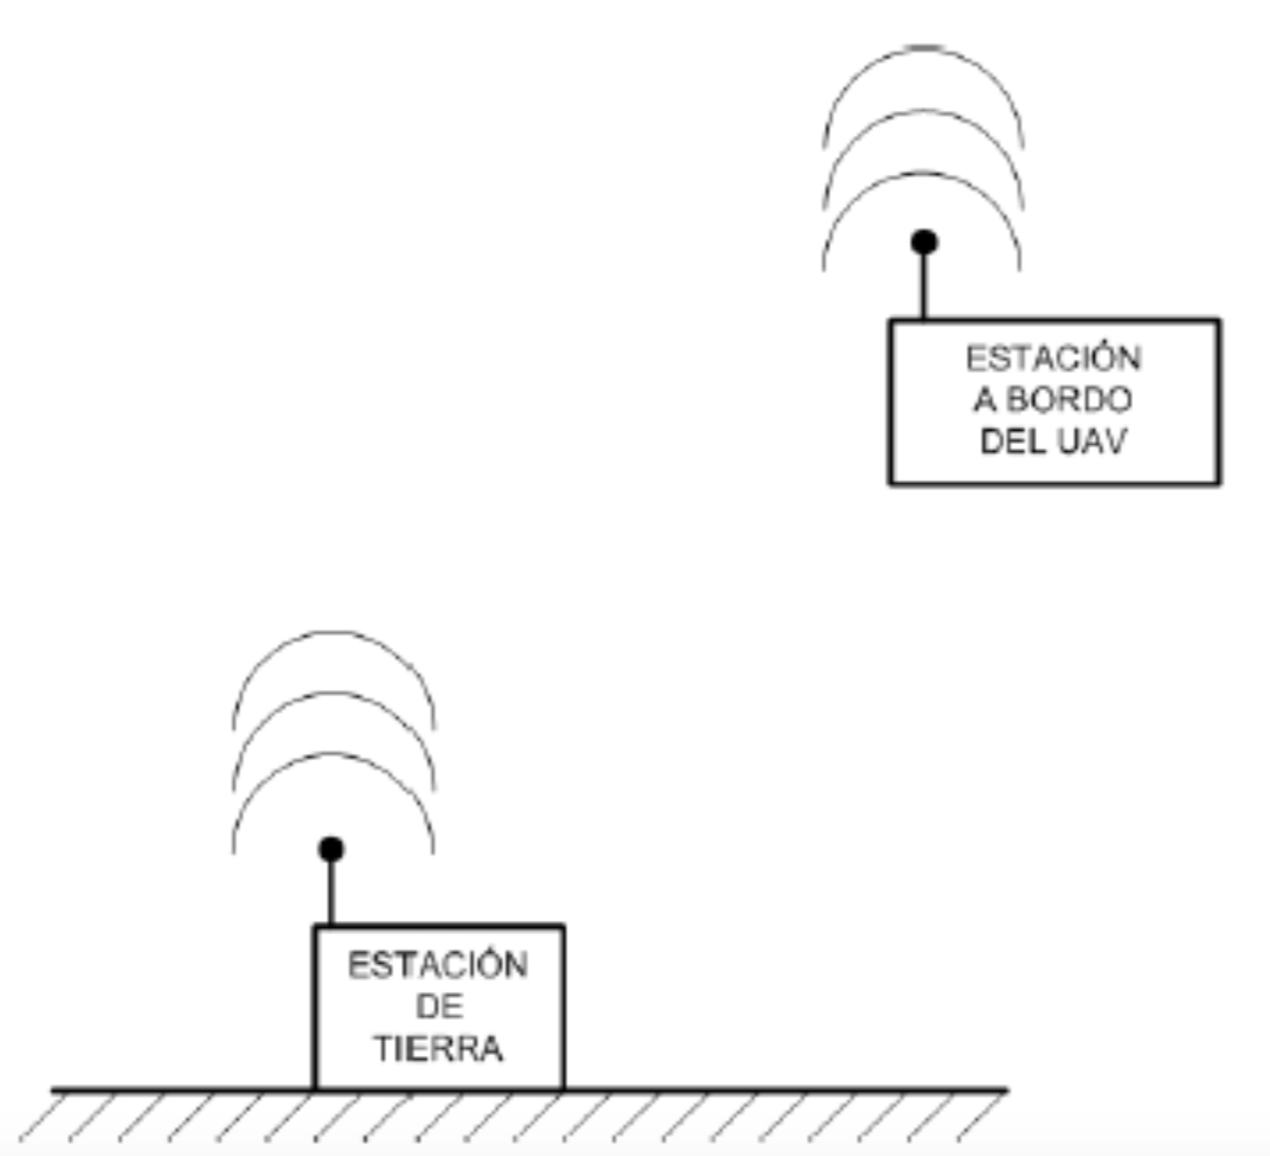
\includegraphics[width=0.8\textwidth]{radiocontrol}
\caption{Sistema RC para estaciones UAV}
\label{fig:radiocontrol}
\end{figure}


La comunicación entre receptor y transmisor se efectúa mediante radiofrecuencia, existiendo diferentes sistemas de emisión, como AM, FM o 2.4Ghz con diferentes tipo de codificación, PCM, PPM…\\

Estos sistemas tienen varias limitaciones. Una es el número de canales máximo del sistema, ya que se usa un canal para cada elemento de control disponible: elevación, giro, rotación… La segunda y posiblemente más crítica son las interferencias. Si se producen interferencias ya sea por ruido o por varios emisores trabajando en las cercanías se puede perder el control de la aeronave produciendo una posible colisión, destruir la misma o incluso dañar a personas.\\
 
\subsection{Sistemas alternativos}

En la actualidad a parte del radiocontrol tenemos el control a través de WiFi. Este sistema consiste en la creación de una red WiFi por parte del drone a la cual se conecta el dispositivo con el que se maneja. Este dispositivo puede ser un mando diseñado y comercializado por la propia marca o un dispositivo móvil, el cuál usa una aplicación que es la que gestiona la conexión y transferencia de datos.\\

La ventaja de estos sistemas es e ahorro de bateria, ya que los transmisores y antenas WiFi necesitan de menos potencia para cubrir las mismas distancias que los sistemas tradicionales de radiocontrol. Además el anocho de banda que nos proporciona es bastante elevado y podremos rtansferir tanto datos como las imágenes de las camaras HD a bordo del drone.\\

Empresas como DJI usa sistemas mixtos que consisten en teleoperar el drone vía radiocontrol, pero la gestión de la cámara, con visualización incluida se realiza mediante una conexión WiFi como la explicada anteriormente.\\
 
La empresa francesa Parrot, la cual tiene una flota de diversos modelos de drones, utiliza un sistema de red WiFi, a la cuál conectas un dispositivo móvil ya sea Android o iOS, y mediante una aplicación desarrollada por ellos se puede teleoperar el drone, así como tener otras funcionalidades como la grabación de video, captura de imágenes y gestión de parámetros de vuelo como altura o velocidad máxima. En capítulos posteriores profundizaremos en este sistema implementado, ya que es el que usaremos para desarrollar el nuestro.\\
 
\section{Tecnologías de comunicación a distancia en tiempo real}

Dentro de las tecnoligías que nos brindan comunicación en timpo real vamos a centrarnos en las que nos ofrecen conectividad multimedia.\\

\subsection{RTP, Protocolo de transporte en tiempo real}

\emph{RTP} son las siglas de \emph{Real-time Transport Protocol}, el cuál es un protocolo de nivel de sesión utilizado para la transmisión de información en tiempo real, como por ejemplo audio, vídeo y datos. Está desarrollado por el grupo de trabajo de transporte de auido y video del IETF (\textbf{Internet Engineering Task Force}). Este protocilo es la base de la industria de Voz sobre IP (\emph{VoIP}).\\

RTP se encapsula sobre UDP y usa un puerto de usuario para cada medio que transfiere, admite direcciones de destino tanto \emph{unicast} como \emph{multicast}. Se encarga de enciar cualquier tipo de trama generada por cualquier algoritmo de codificación como H261, MPEG-1, MPEG-2... pero no añade ningún tipo de fiabilidad ni de calidad del servicio (\emph{QoS}). Lo único que incorpora son marcas de tiempo para evitar el tembleque o \emph{jitter} y la sincronización entre fujos en el destino y numeros de secuencia para detectar pérdidas en un flujo.\\

RTP trabaja junto con otros dos protocolos que lo complementan. El primero es RTCP (\emph{Real time Control Protocol}), protocolo que proporciona información de control sobre la calidad de la transmisión. Transmite paquetes periódicos asociados a cada flujo RTP que incluye los detalles sobre los participantes, si hubiese más de uno, y las estadísticas de pérdidas que permiten el control de flujo y congestión. Según estas estadistas se puede hacer codificación adaptativa para adaptarse al medio. También trabaja sobre UDP y usa un numero de puerto superior al que usa el flujo de RTP.\\

El segundo es RTSP (\emph{Real Time Streaming Protocol}), protocolo que permite realizar un control remoto de sesión de transmisión multimedia. Es un protocolo independiente del protocolo de transnporte, basado en texto que permite recuperar un determinado medio de un sevidor o grabar una multiconferencia.\\


\begin{figure}[htb]
\centering
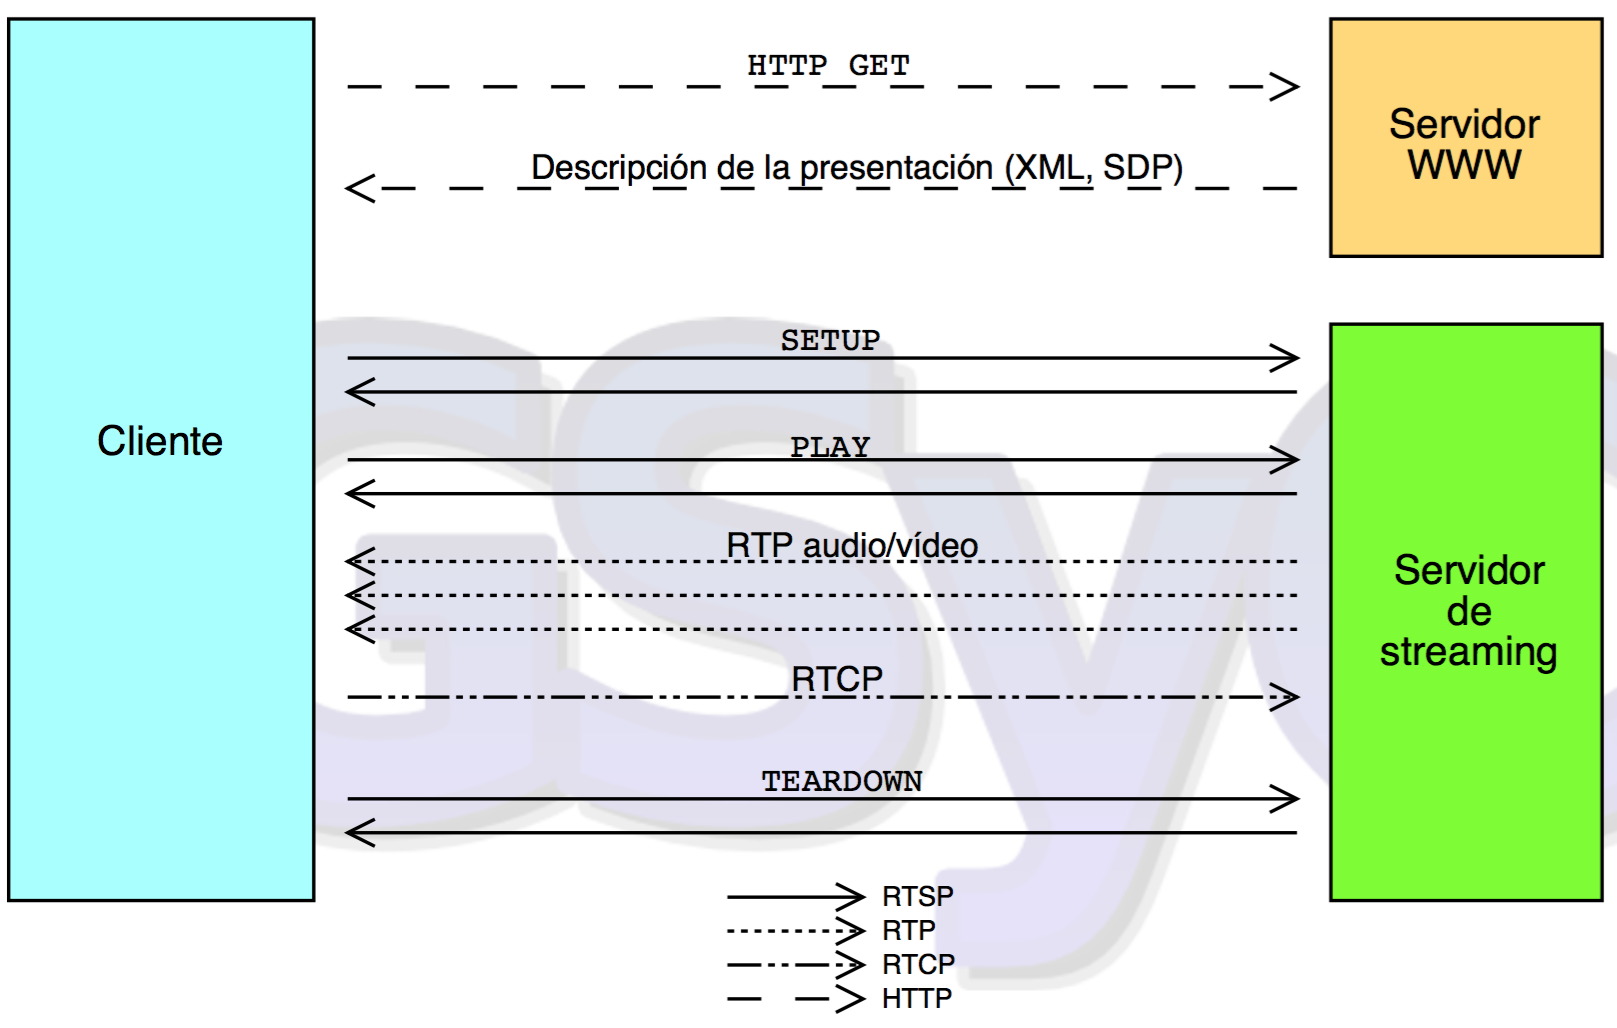
\includegraphics[width=0.8\textwidth]{rtc}
\caption{Ejemplo de conexión RTC, RTCP y RTSP}
\label{fig:rtc}
\end{figure}












\section{Motivación}
